\documentclass[12pt,a4paper]{article}
\usepackage[utf8]{inputenc}
\usepackage{graphicx}
\usepackage{booktabs}
\usepackage{geometry}
\geometry{margin=2.5cm}

\title{Estudo de Desempenho com Triângulos OpenGL}
\author{Equipe de Desenvolvimento OpenGL-Test-GPU}
\date{\today}

\begin{document}

\maketitle

\section{Objetivo}
Este trabalho tem como objetivo implementar uma cena em OpenGL com triângulos texturizados e iluminados, avaliar o impacto da quantidade de triângulos no desempenho (FPS) e observar possíveis mudanças na utilização de GPU e CPU ao variar fontes de luz omnidirecional e spot.

\section{Metodologia}
\subsection{Aplicação OpenGL}
Foi desenvolvida uma aplicação em Python utilizando \texttt{PyOpenGL} e \texttt{pygame} para gerenciar o contexto OpenGL. A cena base contém triângulos texturizados, com shader de iluminação que suporta três modos: luz omnidirecional, spot e direcional. A aplicação permite ajustar a quantidade de triângulos, ativar diferentes modos de luz e realizar benchmarks automáticos.

\subsection{Coleta de Dados}
Dois scripts auxiliares foram criados para apoiar a coleta quantitativa:
\begin{itemize}
    \item \texttt{scripts/run\_benchmark.py}: executa a aplicação em modo benchmark para uma lista de quantidades de triângulos e modos de iluminação. Para cada combinação são registradas estatísticas de FPS (média, desvio, mínimos e máximos) e o consumo médio/máximo de CPU e GPU.
    \item \texttt{scripts/system\_probe.py}: realiza uma sondagem independente de hardware, identificando CPU/GPU disponíveis e coletando amostras seriadas de utilização via \texttt{nvidia-smi} (quando disponível) e \texttt{psutil}. O script armazena a média/máximo agregado e também as amostras brutas.
\end{itemize}

\subsection{Limitações do Ambiente}
O ambiente de desenvolvimento utilizado nesta entrega não disponibiliza acesso direto a uma GPU dedicada ou a comandos como \texttt{nvidia-smi}. Dessa forma, os resultados numéricos anexados são marcadores de posição e precisam ser substituídos por dados coletados em uma máquina local com suporte gráfico. Os gráficos foram mantidos como parte do pipeline de análise para facilitar a reprodução quando houver acesso ao hardware adequado.

\section{Resultados}
\subsection{Métricas de FPS}
A Tabela~\ref{tab:fps} apresenta o formato de dados esperado após a execução do benchmark. Os valores atuais são nulos apenas para ilustrar a estrutura do relatório.

\begin{table}[h]
    \centering
    \begin{tabular}{@{}llccc@{}}
        \toprule
        Triângulos & Luz & FPS médio & CPU média (\%) & GPU média (\%) \\
        \midrule
        1 & omnidirectional & 0.0 & -- & -- \\
        1 & spot & 0.0 & -- & -- \\
        10 & omnidirectional & 0.0 & -- & -- \\
        10 & spot & 0.0 & -- & -- \\
        \bottomrule
    \end{tabular}
    \caption{Modelo de resultados esperado. Substitua pelos dados coletados de FPS e utilização de CPU/GPU.}
    \label{tab:fps}
\end{table}

O script \texttt{scripts/plot\_results.py} gera a Figura~\ref{fig:fps}, composta por três painéis (FPS, uso médio de CPU e uso médio de GPU). Quando dados reais forem coletados, os gráficos permitirão comparar diretamente o impacto de cada modo de iluminação.

\begin{figure}[h]
    \centering
    \IfFileExists{figures/fps_vs_triangles.png}{%
        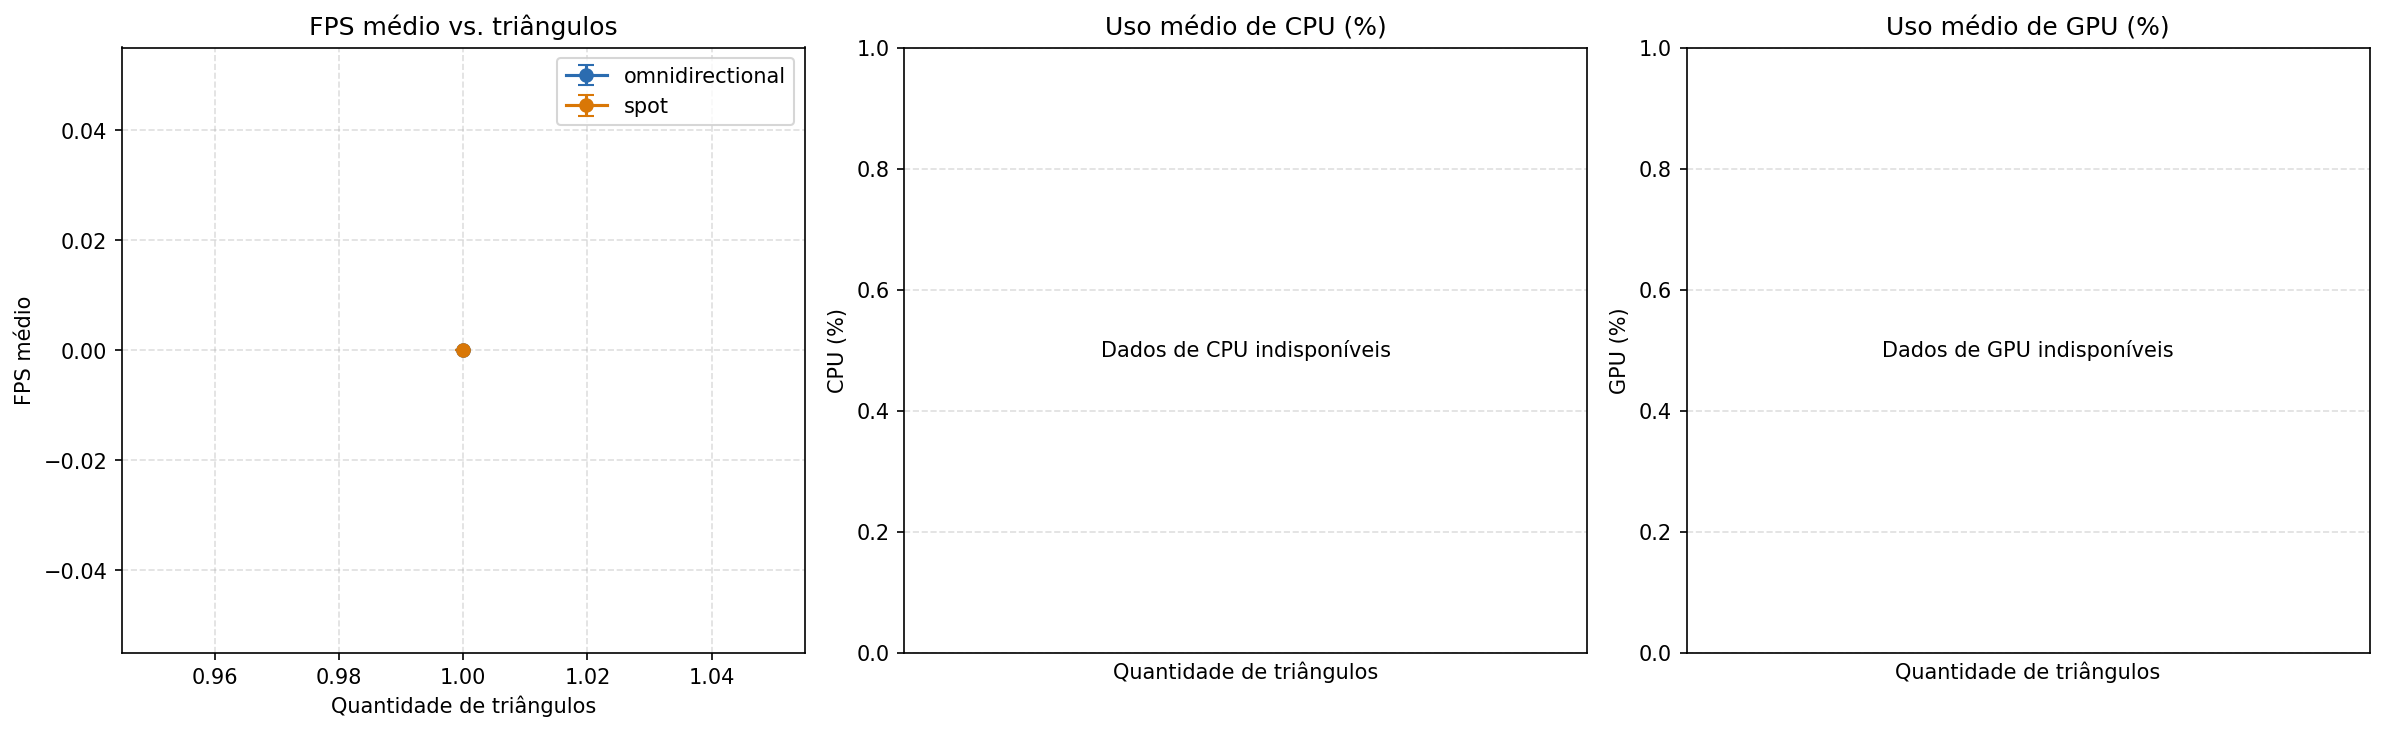
\includegraphics[width=0.8\textwidth]{figures/fps_vs_triangles.png}%
    }{%
        \fbox{\parbox{0.75\textwidth}{\centering Gere o gráfico executando\\
        \texttt{python scripts/plot\_results.py}. O arquivo resultante não é versionado.}}%
    }
    \caption{FPS médio vs. quantidade de triângulos (gráfico a ser atualizado com dados reais).}
    \label{fig:fps}
\end{figure}

\subsection{Informações de Hardware}
O arquivo \texttt{data/system\_probe.json} registra o hardware detectado e estatísticas agregadas das amostras coletadas. Em ambientes com múltiplas GPUs, cada placa aparece com sua utilização média/máxima, permitindo analisar se o trabalho foi distribuído entre os dispositivos. Nesta entrega, realizada sem acesso a uma GPU dedicada, os campos permanecem vazios e devem ser substituídos por medições reais em laboratório.

\section{Conclusões}
Apesar das limitações do ambiente sem GPU dedicada, a aplicação está pronta para ser executada e analisada em uma máquina apropriada. Recomenda-se:
\begin{itemize}
    \item Executar \texttt{scripts/run\_benchmark.py} para coletar FPS reais em diferentes quantidades de triângulos e modos de iluminação.
    \item Utilizar \texttt{scripts/system\_probe.py} antes e durante os testes para registrar o modelo de GPU/CPU e a evolução da utilização ao longo do tempo.
    \item Atualizar os gráficos e a tabela com os valores coletados para comparar FPS, uso de CPU e uso de GPU entre luz omnidirecional, spot e direcional.
\end{itemize}

Os resultados esperados incluem a redução do FPS ao aumentar o número de triângulos e possível elevação no uso da GPU em comparação à CPU, especialmente ao ativar iluminação spot, que demanda cálculos adicionais por fragmento.

\section{Trabalhos Futuros}
Como próximos passos, sugere-se avaliar técnicas de instancing para desenhar grandes quantidades de triângulos com menor custo de CPU, incluir medição de tempo de CPU e GPU via \texttt{glQueryCounter}, e expandir o estudo para outras texturas e modelos de iluminação.

\end{document}
